\documentclass{article}%
\usepackage[T1]{fontenc}%
\usepackage[utf8]{inputenc}%
\usepackage{lmodern}%
\usepackage{textcomp}%
\usepackage{lastpage}%
\usepackage[head=40pt,margin=0.5in,bottom=0.6in]{geometry}%
\usepackage{graphicx}%
%
\title{\textbf{Pemones abandonaron sus trabajos como guías turísticos para buscar oro}}%
\author{El Nacional Web}%
\date{20/11/2018}%
%
\begin{document}%
\normalsize%
\maketitle%
\textbf{URL: }%
http://www.el{-}nacional.com/noticias/economia/pemones{-}abandonaron{-}sus{-}trabajos{-}como{-}guias{-}turisticos{-}para{-}buscar{-}oro\_260487\newline%
%
\textbf{Periodico: }%
EN, %
ID: %
260487, %
Seccion: %
Economía\newline%
%
\textbf{Palabras Claves: }%
Economía\newline%
%
\textbf{Derecho: }%
2.9%
, Otros Derechos: %
3.2%
, Sub Derechos: %
2.9.1, 3.2.1%
\newline%
%
\textbf{EP: }%
NO\newline%
\newline%
%
\textbf{\textit{En Kamarata los comerciantes cobran los productos con oro, pagan el equivalente a ocho dólares en oro por un kilo de arroz}}%
\newline%
\newline%
%
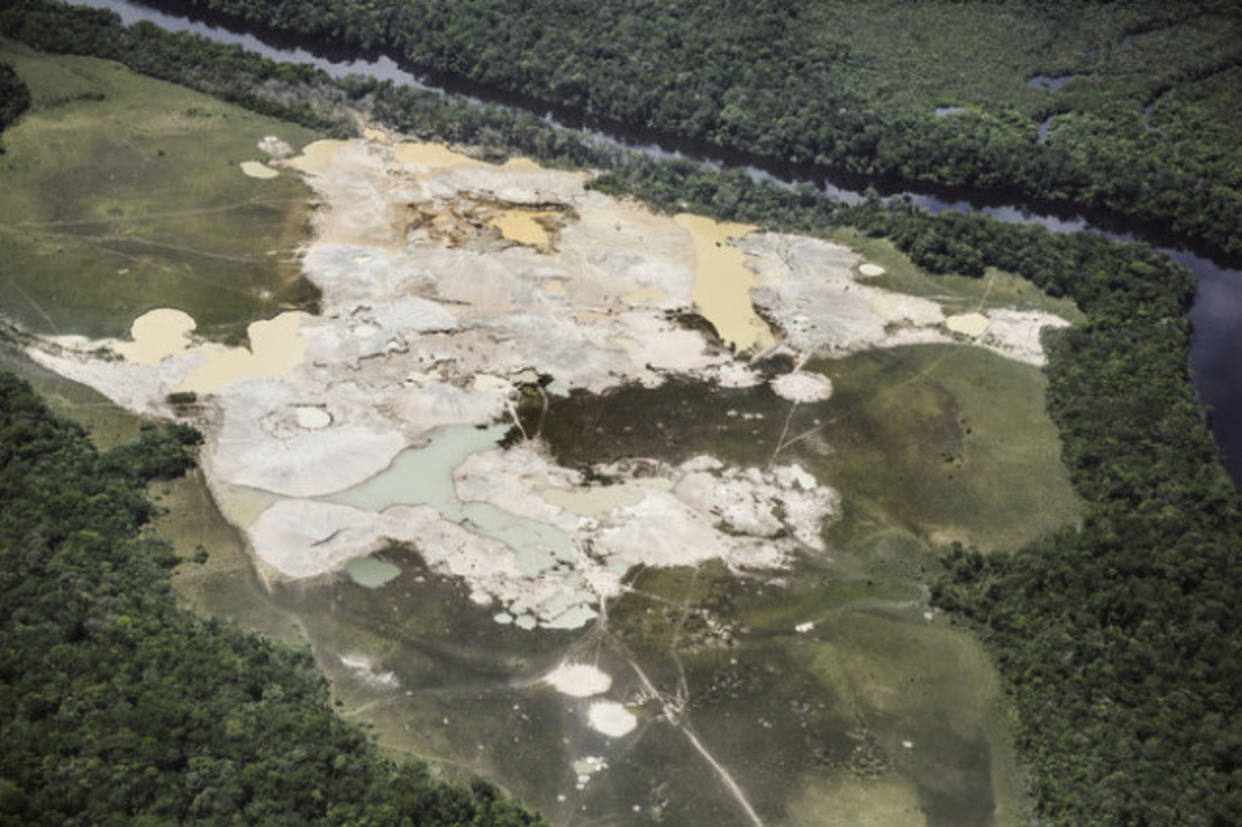
\includegraphics[width=300px]{53.jpg}%
\newline%
%
Los indígenas Pemón han cuidado del Parque Nacional Canaima y del Salto Ángel durante mucho tiempo. Actualmente, la crisis que atraviesa el país, los ha apartado de sus trabajos como guías turísticos para dedicarse a buscar oro.%
\newline%
%
El nuevo trabajo, que los apartó del que tradicionalmente realizaban, deteriora el área por las minas, reseñó~The Wall Street Journal.%
\newline%
%
“Nosotros, los pemones, siempre fuimos ecologistas, los protectores de esta tierra. Pero la situación nos ha convertido en los destructores de nuestro propio hábitat”, dijo Abrahan Sandoval, capitán de la aldea Kamarata.%
\newline%
%
Los comerciantes en Kamarata, donde también hay minería de diamantes y coltán, cobran los artículos con oro. Allí pagan el equivalente a ocho dólares en oro por un kilo de arroz.%
\newline%
%
Con información de~The Wall Street~Journal%
\newline%
%
\end{document}